\documentclass{article}
\usepackage{graphicx}
\usepackage[margin=1.5cm]{geometry}
\usepackage{amsmath}

\begin{document}

\title{Final Exam: Elementary Statistics}
\author{Prof. Jordan C. Hanson}

\maketitle

\section{Formula Area}

\begin{enumerate}
\item Average/mean, definition 1: $\bar{x} = N^{-1} \sum_i x_i$
\item Median: the value below which are half of the frequencies.  Half of the frequencies are also above this value.
\item Mode: the value corresponding to the highest frequendy.
\item The quartiles $Q1$, $Q2$, and $Q3$ are the values that separate the frequencies into four bins of equal frequency. $Q2$ is equal to the median.  The IQR is $Q3 - Q1$.
\item The k-th percentile: the value below which k percent of the data is located.  Formula: $i = (k/100) (n+1)$, where $k$ is the percentile, $n$ is the total number of data, and $i$ is the integer location of the k-th percentile.
\item Finding the percentile of a data value: $(x+0.5*y)/n (100)$, where $x$ is the number of data values below the given data value, $y$ is the number of data values equal to the given one, and $n$ is the total number of data values.
\item Average/mean, definition 2: $\bar{x} = \sum_i^{M} f_{r,i} x_i$, where $x_i$ are the bin centers of a histogram, or the discrete random variable data values, and $f_{r,i}$ are the relative frequencies.  For a discrete random variable, $f_{r,i}$ is replaced with $p(x)$, the probability distribution function.
\item Probabilities of mutually exclusive and independent events: if two events have probabilities $p_1$ and $p_2$, then the probability that event 1 AND event 2 occur is $p_1 p_2$.  The probability that event 1 OR event 2 occurs is $p_1 + p_2$.
\item The standard deviation $s$ of a sample is 
\begin{equation}
s^2 = \frac{1}{N-1}\sum_{i=1}^{M} (x_i-\bar{x})^2
\end{equation}
\item The mean and standard deviation of the binomial distribution are $\mu = np$ and $\sigma = \sqrt{npq}$, respectively.
\item Let the PDF of the \textit{uniform distribution} be $p(x) = 1/(b+a)$.  The mean and standard deviation of this PDF are $\mu = (b+a)/2$ and $\sigma = \sqrt{(b-a)/12}$, respectively.
\item Let the PDF of the \textit{normal distribution} be $p(x) = \frac{1}{\sqrt{2\pi\sigma^2}} \exp(-0.5 (x-\mu)^2/\sigma^2)$.  The mean and standard deviation of this PDF are $\mu$ and $\sigma$, respectively.  We write $N(a,b)$ to refer to a normal distribution with mean $a$ and standard deviation $b$.
\item The z-score of a result drawn from $N(\mu,\sigma)$ is $z = (x_i - \mu)/\sigma$.  $P(|z| \leq 1) \approx 0.68)$, $P(|z| \leq 2) \approx 0.95)$, $P(|z| \leq 1) \approx 0.997)$.
\item \textbf{The central limit theorem} states that the means of samples of a population are distributed according to $N(\bar{x},\sigma_x/\sqrt{n})$, if the sample size is $n$.
\item \textbf{The confidence interval} [a,b] may be constructed such that a fraction CL of all confidence intervals with the same properties will contain the population mean, $\mu$.  The number CL is called the \textit{confidence level.}
\item Given the null hypothesis $H_0$ and an alternative hypothesis $H_a$, a \textbf{Type I error} is when we reject $H_0$ in favor of $H_a$, when $H_0$ is true.
\item Given the null hypothesis $H_0$ and an alternative hypothesis $H_a$, a \textbf{Type II error} is when we accept $H_0$ and reject $H_a$, when $H_0$ is false. 
\end{enumerate}

\clearpage

\begin{figure}[ht]
\centering
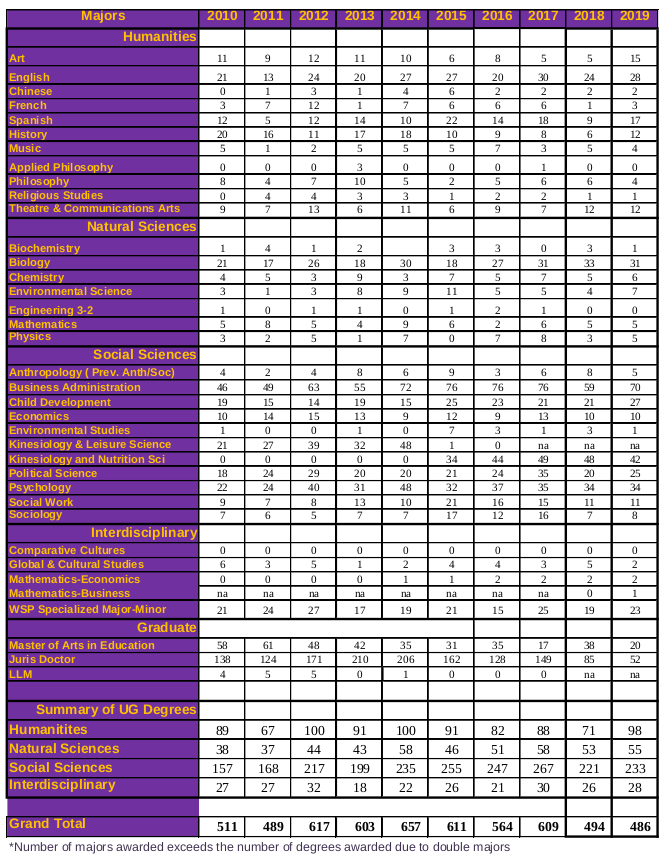
\includegraphics[width=0.8\textwidth]{figures/degree.png}
\caption{\label{fig:degree} Information regarding awarded Whittier College degrees.}
\end{figure}

\clearpage

\begin{enumerate}
\item Consider Fig. \ref{fig:degree}.  (a) Create a histogram of the total degrees per year, with one bin per year. (b) Normalize the frequencies.  (c) Create the \textit{cumulative relative frequency} graph, of the cumulative frequencies.  (d) Repeat this exercise, but for only the degrees awarded in your major.  If you have not selected a major, default to the Whittier Scholars Program (WSP).  \\ \vspace{6cm}
\item Consider Fig. \ref{fig:degree}.  (a) Consider the distribution of social science degrees awarded over the past decade.  What is the 60th percentile for the number of social science degrees awarded?  That is, find the number of degrees below which 60 percent of the results fall. \\ \vspace{3cm}
\item (a) Find the mean number of business administraction degrees awarded per year, and obtain the standard deviation.  Assume that the data is described by a normal distribution, N(mean,std. dev.).  (b) What number of degrees would correspond to a z-score of +3.0? (c) Suppose the same degree data from another department was distributed according to a \textit{uniform distribution.}  If the maximum observed degrees was 25 per year, and the minimum was 15 per year, what would be the average degrees per year?  (How do you get the average of a uniform PDF?)  \\ \vspace{3cm}
\item Suppose a stock price is listed each day, in USD.  Suppose the price is rounded to the nearest dollar in some analysis, and a discrete PDF describes the data well: $p(x) = 1/(x_{max} - x_{min})$.  Let $x_{max} = 30.0$ and $x_{min} = 10.0$.  The prices can therefore be 10, 11, 12, ... , 30.  What is the expectation value of the discrete PDF?  That is, sum $x p(x)$.  \\ \vspace{3cm}
\item A quality control specialist for a restaurant chain takes a
random sample of size 12 to check the amount of soda served in the 16 oz. serving size. The sample mean is 13.30 with a
sample standard deviation of 1.55. Assume the underlying population is normally distributed.  Find the 95\% Confidence Interval for the true population mean for the amount of soda served.
\begin{itemize}
\item A: (12.42, 14.18)
\item B: (12.32, 14.29)
\item C: (12.50, 14.10)
\item D: Cannot determine
\end{itemize}
\item Suppose a new medicine moves ahead with human trials.  When people are given a placebo dose, 10 percent of them are ``cured.''  The fraction of patients cured with the new medicine is $20 \pm 5$ \%.  Suppose we construct a null hypothesis $H_0$: ``If the fraction of patients cured is less than or equal to the result corresponding to one standard deviation above the placebo result, then the drug is ineffective.''  (a) Should we reject or confirm the null hypothesis?  At what significance level is this result? (b) Suppose there was a problem with the data, and the true rate of cure is actually $10 \pm 5$ \%.  What has happened to the significance level of the drug trial?
\end{enumerate}

\end{document}